
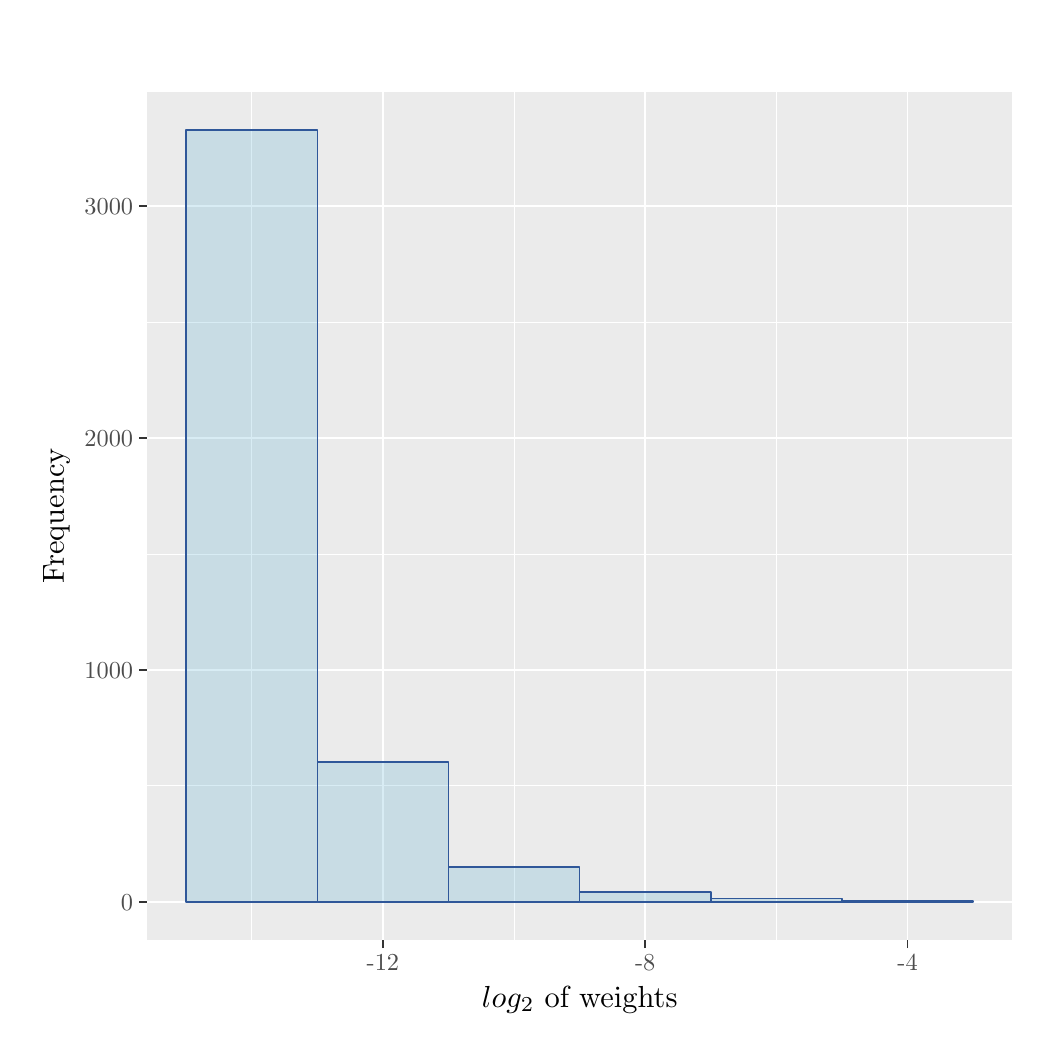
\begin{tikzpicture}[x=1pt,y=1pt]
\definecolor{fillColor}{RGB}{255,255,255}
\path[use as bounding box,fill=fillColor,fill opacity=0.00] (0,0) rectangle (361.35,361.35);
\begin{scope}
\path[clip] (  0.00,  0.00) rectangle (361.35,361.35);
\definecolor{drawColor}{RGB}{255,255,255}
\definecolor{fillColor}{RGB}{255,255,255}

\path[draw=drawColor,line width= 0.6pt,line join=round,line cap=round,fill=fillColor] (  0.00,  0.00) rectangle (361.35,361.35);
\end{scope}
\begin{scope}
\path[clip] ( 43.07, 31.53) rectangle (355.85,338.21);
\definecolor{fillColor}{gray}{0.92}

\path[fill=fillColor] ( 43.07, 31.53) rectangle (355.85,338.21);
\definecolor{drawColor}{RGB}{255,255,255}

\path[draw=drawColor,line width= 0.3pt,line join=round] ( 43.07, 87.37) --
	(355.85, 87.37);

\path[draw=drawColor,line width= 0.3pt,line join=round] ( 43.07,171.17) --
	(355.85,171.17);

\path[draw=drawColor,line width= 0.3pt,line join=round] ( 43.07,254.97) --
	(355.85,254.97);

\path[draw=drawColor,line width= 0.3pt,line join=round] ( 80.98, 31.53) --
	( 80.98,338.21);

\path[draw=drawColor,line width= 0.3pt,line join=round] (175.76, 31.53) --
	(175.76,338.21);

\path[draw=drawColor,line width= 0.3pt,line join=round] (270.55, 31.53) --
	(270.55,338.21);

\path[draw=drawColor,line width= 0.6pt,line join=round] ( 43.07, 45.47) --
	(355.85, 45.47);

\path[draw=drawColor,line width= 0.6pt,line join=round] ( 43.07,129.27) --
	(355.85,129.27);

\path[draw=drawColor,line width= 0.6pt,line join=round] ( 43.07,213.07) --
	(355.85,213.07);

\path[draw=drawColor,line width= 0.6pt,line join=round] ( 43.07,296.87) --
	(355.85,296.87);

\path[draw=drawColor,line width= 0.6pt,line join=round] (128.37, 31.53) --
	(128.37,338.21);

\path[draw=drawColor,line width= 0.6pt,line join=round] (223.15, 31.53) --
	(223.15,338.21);

\path[draw=drawColor,line width= 0.6pt,line join=round] (317.94, 31.53) --
	(317.94,338.21);
\definecolor{drawColor}{RGB}{47,87,153}
\definecolor{fillColor}{RGB}{62,164,201}

\path[draw=drawColor,line width= 0.6pt,line join=round,fill=fillColor,fill opacity=0.20] ( 57.28, 45.47) rectangle (104.67,324.27);

\path[draw=drawColor,line width= 0.6pt,line join=round,fill=fillColor,fill opacity=0.20] (104.67, 45.47) rectangle (152.07, 95.92);

\path[draw=drawColor,line width= 0.6pt,line join=round,fill=fillColor,fill opacity=0.20] (152.07, 45.47) rectangle (199.46, 58.12);

\path[draw=drawColor,line width= 0.6pt,line join=round,fill=fillColor,fill opacity=0.20] (199.46, 45.47) rectangle (246.85, 48.99);

\path[draw=drawColor,line width= 0.6pt,line join=round,fill=fillColor,fill opacity=0.20] (246.85, 45.47) rectangle (294.24, 46.64);

\path[draw=drawColor,line width= 0.6pt,line join=round,fill=fillColor,fill opacity=0.20] (294.24, 45.47) rectangle (341.63, 45.81);
\end{scope}
\begin{scope}
\path[clip] (  0.00,  0.00) rectangle (361.35,361.35);
\definecolor{drawColor}{gray}{0.30}

\node[text=drawColor,anchor=base east,inner sep=0pt, outer sep=0pt, scale=  0.88] at ( 38.12, 42.44) {0};

\node[text=drawColor,anchor=base east,inner sep=0pt, outer sep=0pt, scale=  0.88] at ( 38.12,126.24) {1000};

\node[text=drawColor,anchor=base east,inner sep=0pt, outer sep=0pt, scale=  0.88] at ( 38.12,210.04) {2000};

\node[text=drawColor,anchor=base east,inner sep=0pt, outer sep=0pt, scale=  0.88] at ( 38.12,293.84) {3000};
\end{scope}
\begin{scope}
\path[clip] (  0.00,  0.00) rectangle (361.35,361.35);
\definecolor{drawColor}{gray}{0.20}

\path[draw=drawColor,line width= 0.6pt,line join=round] ( 40.32, 45.47) --
	( 43.07, 45.47);

\path[draw=drawColor,line width= 0.6pt,line join=round] ( 40.32,129.27) --
	( 43.07,129.27);

\path[draw=drawColor,line width= 0.6pt,line join=round] ( 40.32,213.07) --
	( 43.07,213.07);

\path[draw=drawColor,line width= 0.6pt,line join=round] ( 40.32,296.87) --
	( 43.07,296.87);
\end{scope}
\begin{scope}
\path[clip] (  0.00,  0.00) rectangle (361.35,361.35);
\definecolor{drawColor}{gray}{0.20}

\path[draw=drawColor,line width= 0.6pt,line join=round] (128.37, 28.78) --
	(128.37, 31.53);

\path[draw=drawColor,line width= 0.6pt,line join=round] (223.15, 28.78) --
	(223.15, 31.53);

\path[draw=drawColor,line width= 0.6pt,line join=round] (317.94, 28.78) --
	(317.94, 31.53);
\end{scope}
\begin{scope}
\path[clip] (  0.00,  0.00) rectangle (361.35,361.35);
\definecolor{drawColor}{gray}{0.30}

\node[text=drawColor,anchor=base,inner sep=0pt, outer sep=0pt, scale=  0.88] at (128.37, 20.52) {-12};

\node[text=drawColor,anchor=base,inner sep=0pt, outer sep=0pt, scale=  0.88] at (223.15, 20.52) {-8};

\node[text=drawColor,anchor=base,inner sep=0pt, outer sep=0pt, scale=  0.88] at (317.94, 20.52) {-4};
\end{scope}
\begin{scope}
\path[clip] (  0.00,  0.00) rectangle (361.35,361.35);
\definecolor{drawColor}{RGB}{0,0,0}

\node[text=drawColor,anchor=base,inner sep=0pt, outer sep=0pt, scale=  1.10] at (199.46,  7.44) {$log_2$ of weights};
\end{scope}
\begin{scope}
\path[clip] (  0.00,  0.00) rectangle (361.35,361.35);
\definecolor{drawColor}{RGB}{0,0,0}

\node[text=drawColor,rotate= 90.00,anchor=base,inner sep=0pt, outer sep=0pt, scale=  1.10] at ( 13.08,184.87) {Frequency};
\end{scope}
\begin{scope}
\path[clip] (  0.00,  0.00) rectangle (361.35,361.35);
\definecolor{drawColor}{RGB}{0,0,0}


\end{scope}
\end{tikzpicture}

